% !TEX encoding = UTF-8 Unicode
% !TEX spellcheck = de_DE

\section{Aktueller Stand}
\subsection{Hardwareaufbau}

Für die akustische Messung werden sog. MSM, Multi-Sensor Mikrofon, Einheiten genutzt welche bis zu zwei Mikrofone aufweisen können. Abbildung \ref{fig:msmblockdiagram} zeigt das Blockschaltbild einer solchen Einheit.

\begin{figure}[H]
	\centering
	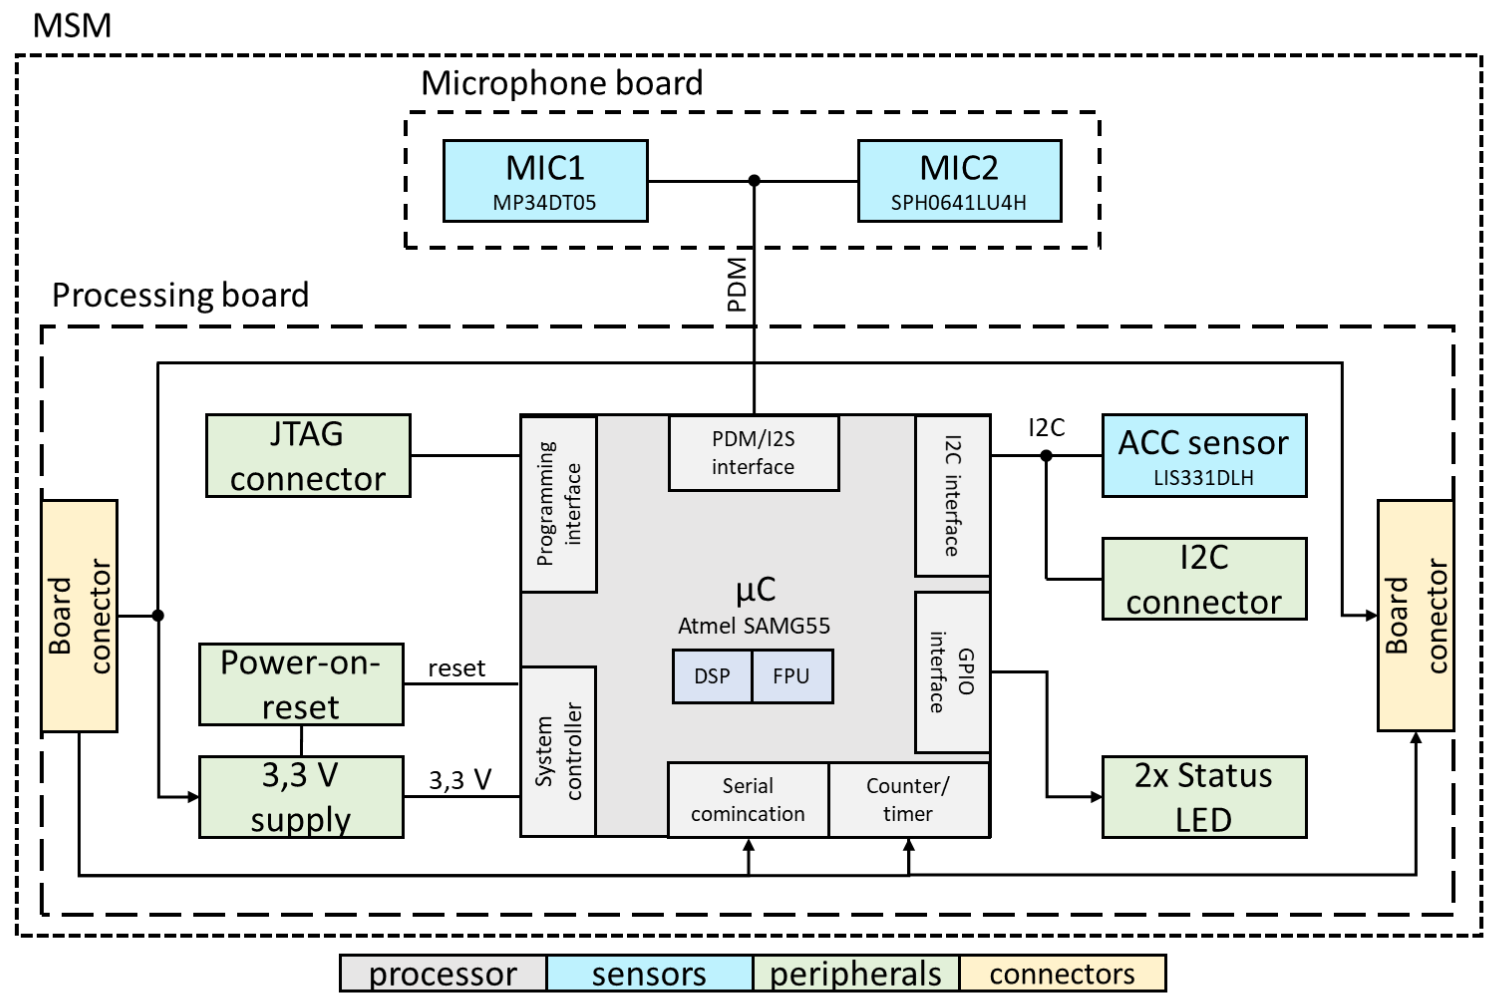
\includegraphics[width=0.7\linewidth]{images/MSM_block_diagram}
	\caption{Blockschaltbild der MSM Einheit}
	\label{fig:msmblockdiagram}
\end{figure}

Die MSM Einheit besteht aus einem Mikrofon Board und einem \glqq Processing board\grqq. Bis zu zwei Mikrofone werden über ein PDM Interface an einen Atmel SAMG55J19 Mikrocontroller angeschlossen. Dieser sorgt für die Kommunikation zur äußeren Umgebung mittels seriellem Interface, welches über die in Gelb dargestellten Board Stecker zugänglich ist. Dabei handelt es sich um den TDM Bus. Zusätzlich verfügt das Processing board über einen Beschleunigungssensor LIS331DLH, welcher derzeit jedoch nicht benutzt wird. Die eingehenden Daten der Mikrofone werden aktuell direkt weitergegeben. Es erfolgt keine Signalverarbeitung.\\
\\
Abbildung \ref{fig:microphone} zeigt wie die MSM Einheit in einem Rohrausschnitt aussieht.

\begin{figure}[H]
	\centering
	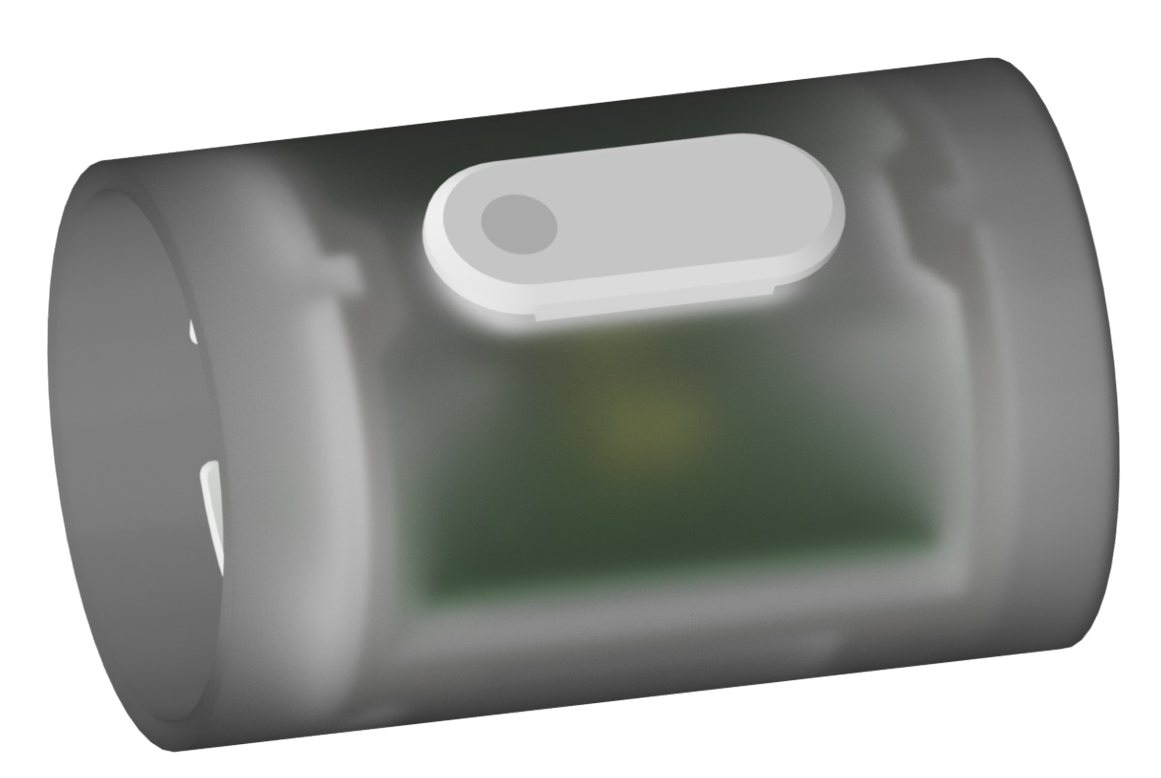
\includegraphics[width=0.4\linewidth]{images/microphone}
	\caption{MSM Einheit in einem Rohrausschnitt}
	\label{fig:microphone}
\end{figure}

\newpage
\subsection{Firmwareablauf}

\begin{figure}[H]
	\centering
	\resizebox{0.55\linewidth}{!}{%
		\begin{tikzpicture}[every text node part/.style={align=center},
		node distance=1.5cm, 
		->, 
		>=stealth', 
		shorten >=1pt, 
		auto]
		
		\node (1) [draw, minimum width=3cm, minimum height=1cm]             {sysclk\_init();};
		\node (2) [draw, minimum width=3cm, minimum height=1cm, below of=1] {board\_init();};
		\node (3) [draw, minimum width=3cm, minimum height=1cm, below of=2] {tc\_waveform\_initialize();};
		\node (4) [draw, minimum width=3cm, minimum height=1cm, below of=3] {init\_pdm();};
		\node (5) [draw, minimum width=3cm, minimum height=1cm, below of=4] {Enable\_global\_interrupt();};
		\node (6) [draw, minimum width=3cm, minimum height=1cm, below of=5] {enable\_pdm();};
		\node (7) [draw, minimum width=3cm, minimum height=1cm, below of=6] {NVIC\_DisableIRQ(SPI\_IRQn);};
		\node (8) [draw, minimum width=3cm, minimum height=1cm, below of=7] {NVIC\_ClearPending(SPI\_IRQn);};
		\node (9) [draw, minimum width=3cm, minimum height=1cm, below of=8] {NVIC\_SetPriority(SPI\_IRQn, 0);};
		\node (10)[draw, minimum width=3cm, minimum height=1cm, below of=9] {NVIC\_EnableIRQ(SPI\_IRQn);};
		\node (11)[draw, minimum width=3cm, minimum height=1cm, below of=10]{spi\_slave\_initialize();};
		\node (12)[draw, minimum width=3cm, minimum height=1cm, below of=11, xshift=3cm, yshift=-1cm]{while(1);};
		
		\node (irq1)[draw, minimum width=3cm, minimum height=1cm, right of=5, xshift=6cm, label={[xshift=-0.7cm]\textit{Interrupt}}]{SPI\_Handler()};
		
		% arrows
		
		\draw [->] (1.south) -- (2.north);
		\draw [->] (2.south) -- (3.north);
		\draw [->] (3.south) -- (4.north);
		\draw [->] (4.south) -- (5.north);
		\draw [->] (5.south) -- (6.north);
		\draw [->] (6.south) -- (7.north);
		\draw [->] (7.south) -- (8.north);
		\draw [->] (8.south) -- (9.north);
		\draw [->] (9.south) -- (10.north);
		\draw [->] (10.south)-- (11.north);
		\draw [->] (11.south)-- ([xshift=-3cm, yshift=0.5cm]12.north) -- ([yshift=0.5cm]12.north) -- (12.north);
		\draw [->] (12.south)-- ([yshift=-0.5cm]12.south) -- ([xshift=3cm, yshift=-0.5cm]12.south) -- ([xshift=3cm, yshift=0.5cm]12.north) -- ([yshift=0.5cm]12.north)node[yshift=-0.02cm]{$\bullet$} -- (12.north);
		
		
		
		\end{tikzpicture}
	}
	\caption{Ablaufplan der Firmware}
	\label{fig:system_concept}
\end{figure}


\textbf{sysclk\_init();}\\
Initialisiert die Systemtaktfrequenz auf 120 MHz\\
\\
\textbf{board\_init();}\\
Initialisiert alle Ein- und Ausgänge, sowie LEDs und Schalter\\
\\
\textbf{tc\_waveform\_initialize();}\\
Initialisiert das \glqq Timer-Counter\grqq~Modul 2, welches als Eingänge, die für den TDM Bus benötigen Signale,  BCLK und LRCLK hat. Genutzt wird dieses Modul zur Erzeugung eines Chip-Selects für das SPI5 Modul. Timer-Counter und SPI Modul agieren zusammen als TDM Modul ermöglichen die Nutzung des TDM Bus.
\newpage
Das TC Modul wird so eingestellt, dass bei jeder fallenden Flanke von BCLK ein interner Zählwert inkrementiert wird. Sobald LRCLK auf eine logische eins gezogen wird, löscht das Timer-Counter Modul den Zählwert und beginnt wieder bei null. Die nachfolgende Abbildung \ref{fig:funktionsweise_tc} zeigt das Verhalten graphisch.

% 60{c} - 60 clock up and downs -> 30 periods
% h or H - high
% l or L - low
% u or U - unknown
% d or D - data, with {} afterwards a name can be given e.g. 10{d}{0x01}
\begin{figure}[H]
	\centering
	\resizebox{0.9\linewidth}{!}{%
	\begin{tikztimingtable}[
		timing/dslope=0.1,
		timing/.style={x=2ex,y=2ex},
		x=2ex,
		timing/rowdist=3ex,
		timing/name/.style={font=\sffamily\scriptsize}
		]
		BCLK & 10{c} 3U 8{c} 3U 10{c}\\
		LRCLK & 1L 1H 3L 3U 4L 3U 2L 1H 2L\\
		Count & 2{d}{63} 2{d}{0} 2{d}{1} 2{d}{2} 2{d}{3} 3U 2{d}{30} 2{d}{31} 2{d}{32} 2{d}{33} 3U 2{d}{62} 2{d}{63} 2{d}{0} 2{d}{1} 2{d}{2}\\
		TDM Slave 0 - TIOA & 2L 3H 3U 2H 2L 3U 3L 2H\\
		TDM Slave 1 - TIOA & 2H 3L 3U 2L 2H 3U 3H 2L\\
		\extracode
		\begin{pgfonlayer}{background}
			\begin{scope}[semitransparent ,semithick]
				\vertlines[darkgray,dotted]{0,1 ,...,20.0}
			\end{scope}
		\end{pgfonlayer}
		
	\end{tikztimingtable}
	}
	\caption{Funktionsweise Timer-Counter Modul}
	\label{fig:funktionsweise_tc}
\end{figure}

Sowie der Zählwert 32 erreicht wird je nach Slave Einstellung das Spannungsniveau von TIOA umgekehrt.\\
\\
Abbildung \ref{fig:interaction_tc_and_spi} zeigt die Verbindung zwischen dem Timer-Counter und SPI Modul. Genutzt wird von drei möglichen Timer-Counter Modulen das dritte Modul TC2 und von acht SPI Modulen das sechste, SPI5. Über die Pins PA21 und PA11 ist der Ausgang von TC2 mit dem Chip-Select Eingang von SPI5 verbunden.

\begin{figure}[H]
	\centering
	\resizebox{0.9\linewidth}{!}{%
		\begin{tikzpicture}[every text node part/.style={align=center},
		node distance=5cm, 
		->, 
		>=stealth', 
		shorten >=1pt, 
		auto]
		
		\node (MSM) [draw, thick, minimum width=7cm, minimum height=10cm, yshift=-2.5cm, label={[xshift=-2.8cm]\textbf{MSM}}]{};
		\node (TC2) [draw, minimum width=3cm, minimum height=4cm, label={[yshift=-0.6cm]TC2}]{};
		\node (SPI5)[draw, minimum width=3cm, minimum height=4cm, below of=TC2, label={[yshift=-0.6cm]SPI5}]{};
		
		%Pins
		\node (pa19)[draw, rounded corners=0.2cm, minimum width=1cm, minimum height=0.5cm, left of=TC2, yshift= 1cm]{PA19};
		\node (pa20)[draw, rounded corners=0.2cm, minimum width=1cm, minimum height=0.5cm, left of=TC2]{PA20};
		\node (pa21)[draw, rounded corners=0.2cm, minimum width=1cm, minimum height=0.5cm, left of=TC2, yshift=-1cm]{PA21};
		
		\node (pa11)[draw, rounded corners=0.2cm, minimum width=1cm, minimum height=0.5cm, left of=SPI5, yshift=0.5cm]{PA11};
		\node (pa14)[draw, rounded corners=0.2cm, minimum width=1cm, minimum height=0.5cm, left of=SPI5, yshift=-0.5cm]{PA14};
		\node (pa12)[draw, rounded corners=0.2cm, minimum width=1cm, minimum height=0.5cm, right of=SPI5]{PA12};
				
		%Lines
		\draw[-]([yshift=1cm]TC2.west)node[label={[xshift=0.4cm, yshift=-0.4cm]\scriptsize{XC1}}]{} -- (pa19.east);
		\draw[-](TC2.west)node[label={[xshift=0.4cm, yshift=-0.4cm]\scriptsize{XC2}}]{} -- (pa20.east);
		\draw[-](TC2.east)node[label={[xshift=-0.5cm, yshift=-0.4cm]\scriptsize{TIOA2}}]{} -- ([xshift=1cm]TC2.east) -- ([xshift=1cm, yshift=-2.5cm]TC2.east) -- ([xshift=2cm, yshift=-1.5cm]pa21.east) -- ([xshift=2cm]pa21.east) -- (pa21.east);
		
		\draw[-]([yshift=0.5cm]SPI5.west)node[label={[xshift=0.6cm, yshift=-0.4cm]\scriptsize{NPCS0}}]{} -- (pa11.east); 
		\draw[-]([yshift=-0.5cm]SPI5.west)node[label={[xshift=0.6cm, yshift=-0.4cm]\scriptsize{SPCK}}]{} -- (pa14.east);
		\draw[-](SPI5.east)node[label={[xshift=-0.4cm, yshift=-0.4cm]\scriptsize{MISO}}]{} -- (pa12.west);
		
		\draw[-](pa21.west) -- ([xshift=-0.5cm]pa21.west) -- ([xshift=-0.5cm]pa11.west) -- (pa11.west);
		\draw[-](pa19.west) -- ([xshift=-1cm]pa19.west)node[label={[yshift=-0.4cm]$\bullet$}]{} -- ([xshift=-1cm]pa14.west) -- (pa14.west);
		\draw[-](pa19.west) -- ([xshift=-3cm]pa19.west)node[label={[xshift=0.6cm, yshift=-0.2cm]BCLK}]{};
		\draw[-](pa20.west) -- ([xshift=-3cm]pa20.west)node[label={[xshift=0.77cm, yshift=-0.2cm]LRCLK}]{};
		\draw[-](pa12.east) -- ([xshift=3cm]pa12.east)node[label={[xshift=-0.85cm, yshift=-0.2cm]SDATA}]{};
		

		\end{tikzpicture}
	}
	\caption{Interaktion TC und SPI Modul}
	\label{fig:interaction_tc_and_spi}
\end{figure}

\newpage

\textbf{init\_pdm();}\\
Konfiguriert das PDMIC Modul 0 so, dass die Abtastrate Fs bei 3,072 MHz liegt, der Verstärkungsfaktor bei 1500, die Überabtastrate bei 64 und die Datengrößen der abgetastet Daten am Ende bei 32 Bit liegen. Alle weiteren Einstellungen entsprechen den Standardwerten.\\
\textbf{Enable\_global\_interrupt();}\\
Diese Funktion schaltet Interrupts allgemein ein.\\
\textbf{enable\_pdm();}\\
Aktiviert das zuvor konfigurierte PDMIC0 Modul.\\
\textbf{NVIC\_DisableIRQ(SPI\_IRQn);}\\
\textbf{NVIC\_ClearPending(SPI\_IRQn);}\\
\textbf{NVIC\_SetPriority(SPI\_IRQn, 0);}\\
\textbf{NVIC\_EnableIRQ(SPI\_IRQn);}\\
Die genannten vier Funktionen aktivieren die Peripheral ID 21, welche dem SPI5 Modul zugehörig ist, als Interruptquelle für den Nested Vector Interrupt Controler (NVIC).\\
\textbf{spi\_slave\_initialize();}\\
Konfiguriert das SPI5 Modul so, dass es im Slave Modus betrieben wird. Mit einer Taktpolarität von 0 und einer Phase von 1 wird auf steigenden Flanken vom Takt ein ausgehendes Datenbit gesetzt. Die Datentransfergröße wird auf acht Bit eingestellt. Abschließend wird das Modul eingeschaltet und die steigende Flanke auf der Chip-Select Leitung als Interrupt-Quelle angegeben. Somit überträgt das SPI Modul Daten wenn durch das Timer-Counter Modul TIOA auf eine logische eins gesetzt wird.

\newpage
\subsection{Mikrofonverhalten}

Um die Mikrofone vor Umwelteinflüssen zu schützen, werden dünne Membranen über den Mikrofonen angebracht. Diese sind abschließend mit der Rohröffnung, sodass kein Schmutz oder Wasser in das Rohr eindringen kann. Die Membranen bestehen aus einem leicht elastischen Thermoplasten und werden in verschiedenen Dicken hergestellt. Abbildung \ref{fig:membranefft} zeigt das Frequenzverhalten eines Mikrofons unter Einfluss der verschiedenen Membranen und ohne Membran.

\begin{figure}[H]
	\centering
	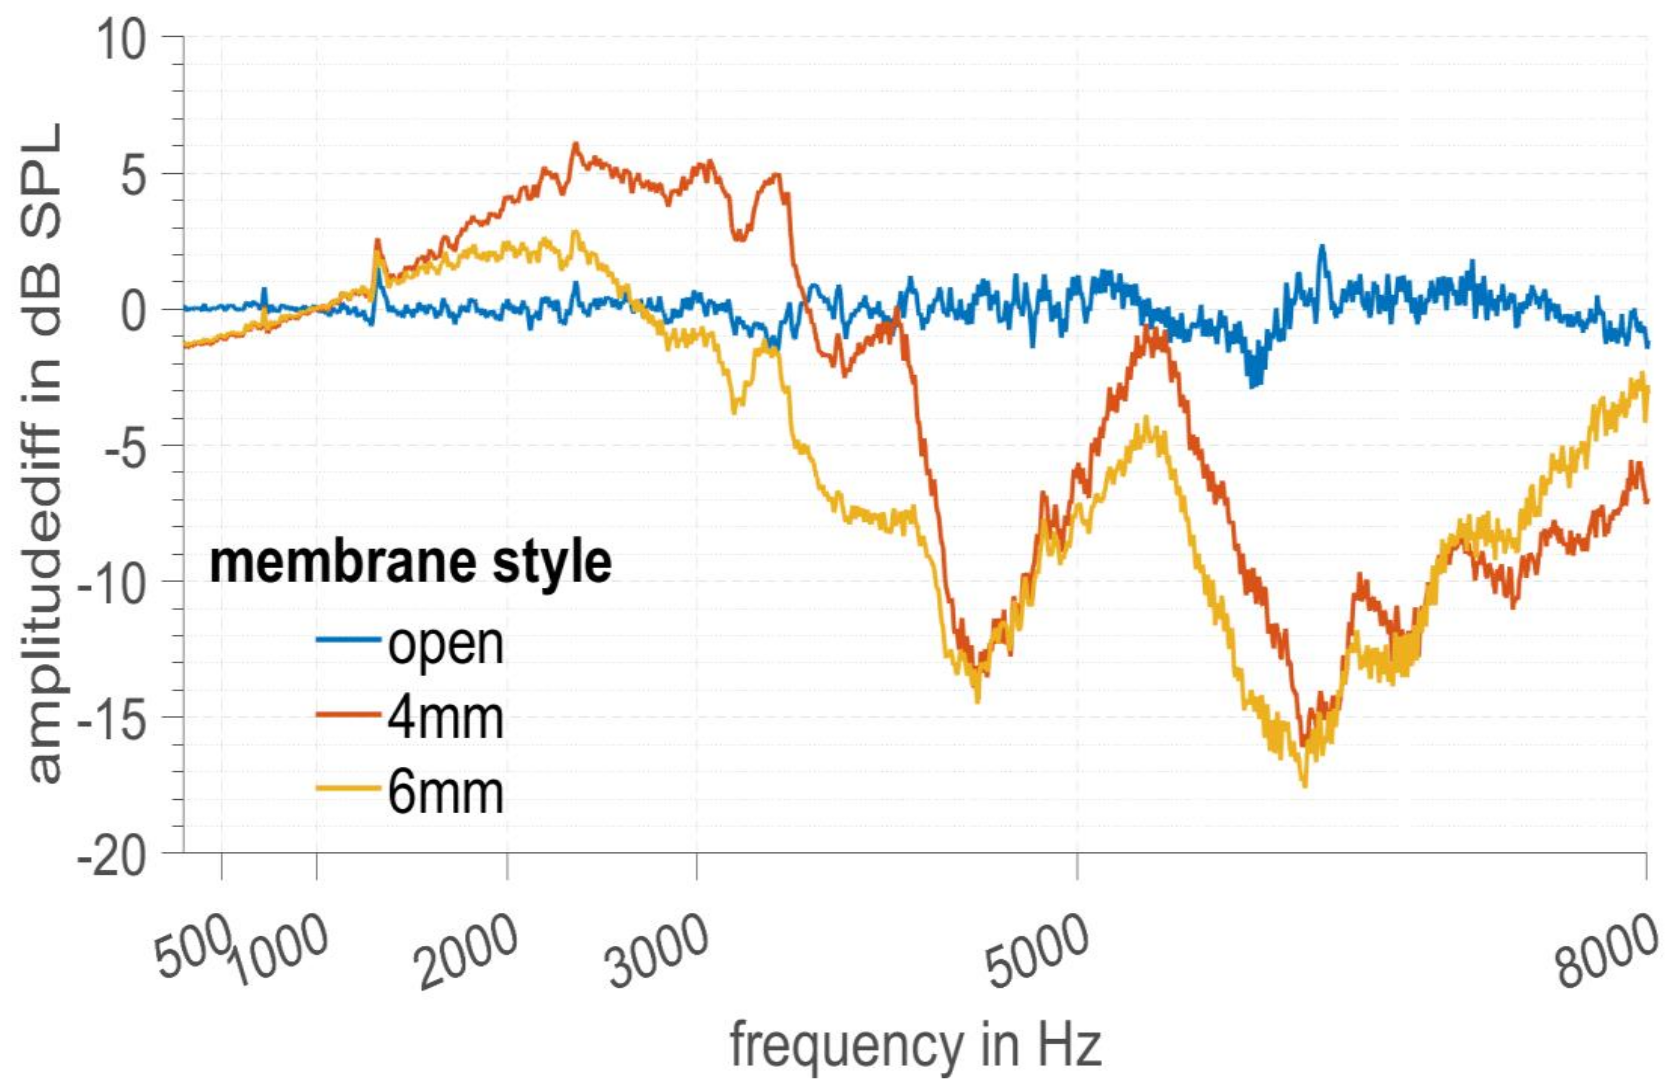
\includegraphics[width=0.9\linewidth]{images/membrane_fft}
	\caption{FFTs verschiedener Membran-Anordnungen}
	\label{fig:membranefft}
\end{figure}

Für diese Messung wird ein Ton einer festen Amplitude auf das Mikrofon gegeben. Die Frequenz dieses Tons wird dabei stets inkrementiert, sodass Frequenzen von etwa 100 Hz bis 8 kHz abgetastet werden. Deutlich zu erkennen ist, dass die Membranen den konstanten Durchlassbereich der Mikrofone, welche diese ohne Membran aufweisen, verändern.

\newpage
\section{Ziele}

Das veränderte Verhalten der Mikrofone durch die Nutzung einer Membran soll mit einem Filterentwurf linearisiert werden. Dafür steht auf dem Atmel SAMG55J19 Mikrocontroller eine DSP Einheit zur Verfügung.

\section{Analyse}

Für eine Membran mit einer Dicke von 6 mm ergibt sich bis 1000 Hz eine Dämpfung von maximal etwa 1,2 dB. Zwischen 1 kHz und 2,8 kHz erfolgt eine Verstärkung mit maximal 3 dB und für den restlichen Frequenzbereich bis 8 kHz entstehen Dämpfungen bis zu 18 dB. Eine maximale Dämpfung von 18 dB entspricht ungefähr dem Faktor von 64, welches einem binären schieben um 6 Stellen nach links gleicht.

\section{Konzept}

Wird das Verhalten der Mikrofone, mit beispielsweise einer 6 mm Membran, linearisiert ergibt sich folgender Graph welcher in Abbildung \ref{fig:matlab1} zu erkennen ist.

\begin{figure}[H]
	\centering
	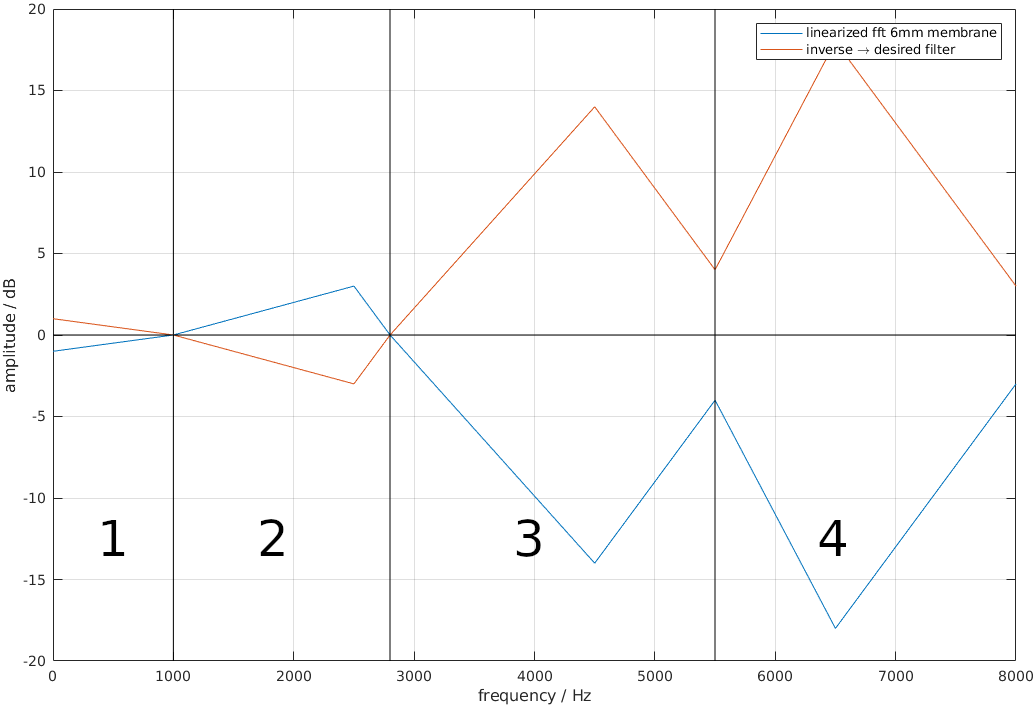
\includegraphics[width=0.9\linewidth]{../../filter_design/matlab/matlab_1}
	\caption{Linearisierte FFT der 6mm Membran und die Inverse}
	\label{fig:matlab1}
\end{figure}

Damit das durch die Membran veränderte Verhalten korrigiert werden kann, muss das zu bauende Filter eine Kennlinie gleich dem Inversen aufweisen. Dieses ist in Abbildung \ref{fig:matlab1} mit der Orangen Linie gekennzeichnet. Ein solches Verhalten ist mit nur einem Filter kaum realisierbar, somit wird die gezeigte Kennlinie in vier Teilbänder unterteilt. Für diese werden nun Filter realisiert. Die Kaskadierung aller vier Teilfilter muss am Ende die Orange Kennlinie wiederspiegeln.


\newpage
\section{Durchführung}

Wie wird eine FFT berechnet?

Basically implement an audio equalizer!

\newpage
\section{Fazit}


\newpage
\section{Ausblick}
